\begin{frame}{Quantitative}
    \begin{itemize}
      \item Our method was compared to the generative models baselines trained to perform the task end-to-end.
      \item Fréchet Inception Distance (FID) \cite{DBLP:journals/corr/HeuselRUNKH17} metric was used for evaluation.
      \item Each configuration was trained $\times 10$ times and the mean and std were used for comparison.
    \end{itemize}
    \begin{table}
        \centering
        \begin{tabular}{| c  c  || c  c |}
            % \toprule
            \multicolumn{2}{c}{Configuration} & \multicolumn{2}{c}{FID} \\
            % \hline\hline
            \hline
            % \midrule
            Backbone & Caption & Mean & Std\\
            \hline
            \multirow{2}{4em}{CycleGan}  & end-to-end    & 51.05             & 9.82\\      
                                         & PETIT (ours)       & \textbf{33.8}     & \textbf{1.23}\\
            \hline
            \multirow{2}{4em}{CUT}       & end-to-end    & 38.43             & 1.52\\
                                         & PETIT (ours)       & \textbf{27.35}    & \textbf{1.01}\\
            \hline
            % \bottomrule
        \end{tabular}
    \end{table}    
\end{frame}

\begin{frame}{Qualitative}
    \begin{figure}
        % 1st Row
        \centering
        \begin{subfigure}[b]{0.185\textwidth}
            \centering
            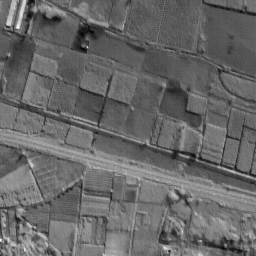
\includegraphics[width=\textwidth]{../figs/outputs/pan/71.png}
        \end{subfigure}
        \hspace{0.05em}%
        \begin{subfigure}[b]{0.185\textwidth}
            \centering
            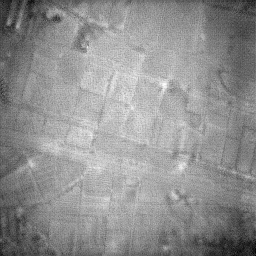
\includegraphics[width=\textwidth]{../figs/outputs/cut/71.png}
        \end{subfigure}
        \hspace{0.05em}%
        \begin{subfigure}[b]{0.185\textwidth}
            \centering
            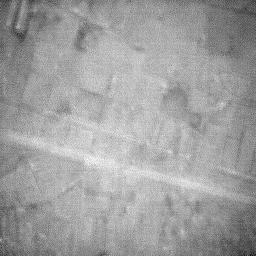
\includegraphics[width=\textwidth]{../figs/outputs/petit/71.png}
        \end{subfigure}
        \hspace{0.05em}%
        \begin{subfigure}[b]{0.185\textwidth}
            \centering
            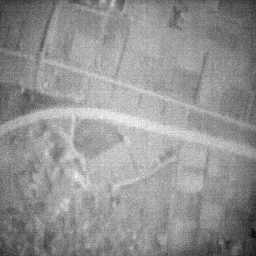
\includegraphics[width=\textwidth]{../figs/outputs/mono/605.png}
        \end{subfigure}      
                
        % 2nd Row
        \begin{subfigure}[b]{0.185\textwidth}
            \centering
            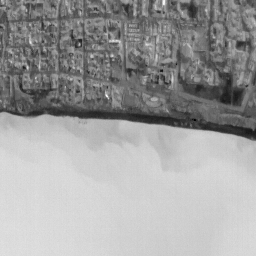
\includegraphics[width=\textwidth]{../figs/outputs/pan/28.png}
            \subcaption*{Pan (input)}
            \label{fig:pan}
        \end{subfigure}
        \hspace{0.05em}%
        \begin{subfigure}[b]{0.185\textwidth}
            \centering
            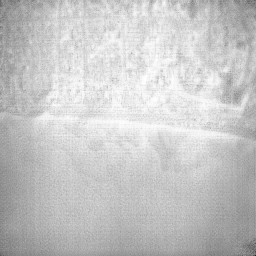
\includegraphics[width=\textwidth]{../figs/outputs/cut/28.png}
            \subcaption*{CUT (baseline)}
            \label{fig:cut}
        \end{subfigure}
        \hspace{0.05em}%
        \begin{subfigure}[b]{0.185\textwidth}
            \centering
            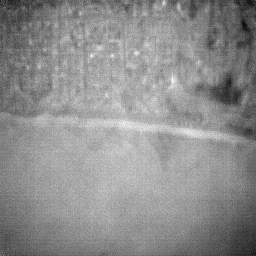
\includegraphics[width=\textwidth]{../figs/outputs/petit/28.png}
            \subcaption*{PETIT (ours)}
            \label{fig:petit}
        \end{subfigure}
        \hspace{0.05em}%
        \begin{subfigure}[b]{0.185\textwidth}
            \centering
            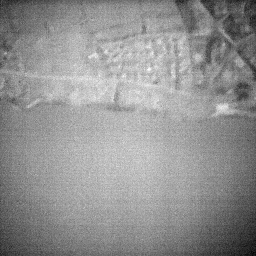
\includegraphics[width=\textwidth]{../figs/outputs/mono/994.png}
            \subcaption*{Mono (ref)}
            \label{fig:mono}
        \end{subfigure}
    
        \label{fig:qual_comp}
    
    \end{figure}
\end{frame}